\documentclass[12pt,twoside]{article}

\usepackage{subfig}
\newcommand{\reporttitle}{CO417 Advance Computing Graphics}
\newcommand{\reportauthor}{Yuan Zhu (Part 1,2) \\Jinwei Zhang (Part 3,4)}
\newcommand{\reporttype}{Assignment 2}

%%%%%%%%%%%%%%%%%%%%%%%%%%%%%%%%%%%%%%%%%
% University Assignment Title Page 
% LaTeX Template
% Version 1.0 (27/12/12)
%
% This template has been downloaded from:
% http://www.LaTeXTemplates.com
%
% Original author:
% WikiBooks (http://en.wikibooks.org/wiki/LaTeX/Title_Creation)
%
% License:
% CC BY-NC-SA 3.0 (http://creativecommons.org/licenses/by-nc-sa/3.0/)
% 
% Instructions for using this template:
% This title page is capable of being compiled as is. This is not useful for 
% including it in another document. To do this, you have two options: 
%
% 1) Copy/paste everything between \begin{document} and \end{document} 
% starting at \begin{titlepage} and paste this into another LaTeX file where you 
% want your title page.
% OR
% 2) Remove everything outside the \begin{titlepage} and \end{titlepage} and 
% move this file to the same directory as the LaTeX file you wish to add it to. 
% Then add \input{./title_page_1.tex} to your LaTeX file where you want your
% title page.
%
%----------------------------------------------------------------------------------------
%	PACKAGES AND OTHER DOCUMENT CONFIGURATIONS
%----------------------------------------------------------------------------------------
\usepackage{tabu}  


\usepackage{ifxetex}
\usepackage{textpos}
\usepackage{natbib}
\usepackage{kpfonts}
\usepackage[a4paper,hmargin=2.8cm,vmargin=2.0cm,includeheadfoot]{geometry}
\usepackage{ifxetex}
\usepackage{stackengine}
\usepackage{tabularx,longtable,multirow,subfigure,caption}%hangcaption
\usepackage{fncylab} %formatting of labels
\usepackage{fancyhdr}
\usepackage{color}
\usepackage[tight,ugly]{units}
\usepackage{url}
\usepackage{float}
\usepackage[english]{babel}
\usepackage{amsmath}
\usepackage{caption}
\usepackage{subfigure}
\usepackage{graphicx}
\usepackage[colorinlistoftodos]{todonotes}
\usepackage{dsfont}
\usepackage{epstopdf} % automatically replace .eps with .pdf in graphics
\usepackage{natbib}
\usepackage{backref}
\usepackage{array}
\usepackage{latexsym}
\usepackage{etoolbox}
\usepackage{bm}

\usepackage{algorithm}  
\usepackage{algpseudocode}  
\usepackage{amsmath}  
\renewcommand{\algorithmicrequire}{\textbf{Input:}}  % Use Input in the format of Algorithm  
\renewcommand{\algorithmicensure}{\textbf{Output:}} % Use Output in the format of Algorithm  

\usepackage{enumerate} % for numbering with [a)] format 

\floatname{algorithm}{Algorithm}  
\renewcommand{\algorithmicrequire}{\textbf{Input:}}  
\renewcommand{\algorithmicensure}{\textbf{Output:}}  

\ifxetex
\usepackage{fontspec}
\setmainfont[Scale=.8]{OpenDyslexic-Regular}
\else
\usepackage[pdftex,pagebackref,hypertexnames=false,colorlinks]{hyperref} % provide links in pdf
\hypersetup{pdftitle={},
  pdfsubject={}, 
  pdfauthor={\reportauthor},
  pdfkeywords={}, 
  pdfstartview=FitH,
  pdfpagemode={UseOutlines},% None, FullScreen, UseOutlines
  bookmarksnumbered=true, bookmarksopen=true, colorlinks,
    citecolor=black,%
    filecolor=black,%
    linkcolor=black,%
    urlcolor=black}
\usepackage[all]{hypcap}
\fi

\usepackage{tcolorbox}

% various theorems
\usepackage{ntheorem}
\theoremstyle{break}
\newtheorem{lemma}{Lemma}
\newtheorem{theorem}{Theorem}
\newtheorem{remark}{Remark}
\newtheorem{definition}{Definition}
\newtheorem{proof}{Proof}

% example-environment
\newenvironment{example}[1][]
{ 
\vspace{4mm}
\noindent\makebox[\linewidth]{\rule{\hsize}{1.5pt}}
\textbf{Example #1}\\
}
{ 
\noindent\newline\makebox[\linewidth]{\rule{\hsize}{1.0pt}}
}



%\renewcommand{\rmdefault}{pplx} % Palatino
% \renewcommand{\rmdefault}{put} % Utopia

\ifxetex
\else
\renewcommand*{\rmdefault}{bch} % Charter
\renewcommand*{\ttdefault}{cmtt} % Computer Modern Typewriter
%\renewcommand*{\rmdefault}{phv} % Helvetica
%\renewcommand*{\rmdefault}{iwona} % Avant Garde
\fi

\setlength{\parindent}{0em}  % indentation of paragraph

\setlength{\headheight}{14.5pt}
%\pagestyle{fancy}
\fancyfoot[ER,OL]{\thepage}%Page no. in the left on
                                %odd pages and on right on even pages
\fancyfoot[OC,EC]{\sffamily }
\renewcommand{\headrulewidth}{0pt}
\renewcommand{\footrulewidth}{0.1pt}
\captionsetup{margin=10pt,font=small,labelfont=bf}


%--- chapter heading

\def\@makechapterhead#1{%
  \vspace*{10\p@}%
  {\parindent \z@ \raggedright %\sffamily
        %{\Large \MakeUppercase{\@chapapp} \space \thechapter}
        %\\
        %\hrulefill
        %\par\nobreak
        %\vskip 10\p@
    \interlinepenalty\@M
    \Huge \bfseries 
    \thechapter \space\space #1\par\nobreak
    \vskip 0\p@
  }}

%---chapter heading for \chapter*  
\def\@makeschapterhead#1{%
  \vspace*{10\p@}%
  {\parindent \z@ \raggedright
    \sffamily
    \interlinepenalty\@M
    \Huge \bfseries  
    #1\par\nobreak
    \vskip 0\p@
  }}
  



% %%%%%%%%%%%%% boxit
\def\Beginboxit
   {\par
    \vbox\bgroup
	   \hrule
	   \hbox\bgroup
		  \vrule \kern1.2pt %
		  \vbox\bgroup\kern1.2pt
   }

\def\Endboxit{%
			      \kern1.2pt
		       \egroup
		  \kern1.2pt\vrule
		\egroup
	   \hrule
	 \egroup
   }	

\newenvironment{boxit}{\Beginboxit}{\Endboxit}
\newenvironment{boxit*}{\Beginboxit\hbox to\hsize{}}{\Endboxit}



\allowdisplaybreaks

\makeatletter
\newcounter{elimination@steps}
\newcolumntype{R}[1]{>{\raggedleft\arraybackslash$}p{#1}<{$}}
\def\elimination@num@rights{}
\def\elimination@num@variables{}
\def\elimination@col@width{}
\newenvironment{elimination}[4][0]
{
    \setcounter{elimination@steps}{0}
    \def\elimination@num@rights{#1}
    \def\elimination@num@variables{#2}
    \def\elimination@col@width{#3}
    \renewcommand{\arraystretch}{#4}
    \start@align\@ne\st@rredtrue\m@ne
}
{
    \endalign
    \ignorespacesafterend
}
\newcommand{\eliminationstep}[2]
{
    \ifnum\value{elimination@steps}>0\leadsto\quad\fi
    \left[
        \ifnum\elimination@num@rights>0
            \begin{array}
            {@{}*{\elimination@num@variables}{R{\elimination@col@width}}
            |@{}*{\elimination@num@rights}{R{\elimination@col@width}}}
        \else
            \begin{array}
            {@{}*{\elimination@num@variables}{R{\elimination@col@width}}}
        \fi
            #1
        \end{array}
    \right]
    & 
    \begin{array}{l}
        #2
    \end{array}
    &%                                    moved second & here
    \addtocounter{elimination@steps}{1}
}
\makeatother

%% Fast macro for column vectors
\makeatletter  
\def\colvec#1{\expandafter\colvec@i#1,,,,,,,,,\@nil}
\def\colvec@i#1,#2,#3,#4,#5,#6,#7,#8,#9\@nil{% 
  \ifx$#2$ \begin{bmatrix}#1\end{bmatrix} \else
    \ifx$#3$ \begin{bmatrix}#1\\#2\end{bmatrix} \else
      \ifx$#4$ \begin{bmatrix}#1\\#2\\#3\end{bmatrix}\else
        \ifx$#5$ \begin{bmatrix}#1\\#2\\#3\\#4\end{bmatrix}\else
          \ifx$#6$ \begin{bmatrix}#1\\#2\\#3\\#4\\#5\end{bmatrix}\else
            \ifx$#7$ \begin{bmatrix}#1\\#2\\#3\\#4\\#5\\#6\end{bmatrix}\else
              \ifx$#8$ \begin{bmatrix}#1\\#2\\#3\\#4\\#5\\#6\\#7\end{bmatrix}\else
                 \PackageError{Column Vector}{The vector you tried to write is too big, use bmatrix instead}{Try using the bmatrix environment}
              \fi
            \fi
          \fi
        \fi
      \fi
    \fi
  \fi 
}  
\makeatother

\robustify{\colvec}

%%% Local Variables: 
%%% mode: latex
%%% TeX-master: "notes"
%%% End: 

% quick way of adding a figure
\newcommand{\fig}[3]{
 \begin{center}
 \scalebox{#3}{\includegraphics[#2]{#1}}
 \end{center}
}

%\newcommand*{\point}[1]{\vec{\mkern0mu#1}}
\newcommand{\ci}[0]{\perp\!\!\!\!\!\perp} % conditional independence
\newcommand{\point}[1]{{#1}} % points 
\renewcommand{\vec}[1]{{\boldsymbol{{#1}}}} % vector
\newcommand{\mat}[1]{{\boldsymbol{{#1}}}} % matrix
\newcommand{\R}[0]{\mathds{R}} % real numbers
\newcommand{\Z}[0]{\mathds{Z}} % integers
\newcommand{\N}[0]{\mathds{N}} % natural numbers
\newcommand{\nat}[0]{\mathds{N}} % natural numbers
\newcommand{\Q}[0]{\mathds{Q}} % rational numbers
\ifxetex
\newcommand{\C}[0]{\mathds{C}} % complex numbers
\else
\newcommand{\C}[0]{\mathds{C}} % complex numbers
\fi
\newcommand{\tr}[0]{\text{tr}} % trace
\renewcommand{\d}[0]{\mathrm{d}} % total derivative
\newcommand{\inv}{^{-1}} % inverse
\newcommand{\id}{\mathrm{id}} % identity mapping
\renewcommand{\dim}{\mathrm{dim}} % dimension
\newcommand{\rank}[0]{\mathrm{rk}} % rank
\newcommand{\determ}[1]{\mathrm{det}(#1)} % determinant
\newcommand{\scp}[2]{\langle #1 , #2 \rangle}
\newcommand{\kernel}[0]{\mathrm{ker}} % kernel/nullspace
\newcommand{\img}[0]{\mathrm{Im}} % image
\newcommand{\idx}[1]{{(#1)}}
\DeclareMathOperator*{\diag}{diag}
\newcommand{\E}{\mathds{E}} % expectation
\newcommand{\var}{\mathds{V}} % variance
\newcommand{\gauss}[2]{\mathcal{N}\big(#1,\,#2\big)} % gaussian distribution N(.,.)
\newcommand{\gaussx}[3]{\mathcal{N}\big(#1\,|\,#2,\,#3\big)} % gaussian distribution N(.|.,.)
\newcommand{\gaussBig}[2]{\mathcal{N}\left(#1,\,#2\right)} % see above, but with brackets that adjust to the height of the arguments
\newcommand{\gaussxBig}[3]{\mathcal{N}\left(#1\,|\,#2,\,#3\right)} % see above, but with brackets that adjust to the height of the arguments
\DeclareMathOperator{\cov}{Cov} % covariance (matrix) 
\ifxetex
\renewcommand{\T}[0]{^\top} % transpose
\else
\newcommand{\T}[0]{^\top}
\fi
% matrix determinant
\newcommand{\matdet}[1]{
\left|
\begin{matrix}
#1
\end{matrix}
\right|
}



%%% various color definitions
\definecolor{darkgreen}{rgb}{0,0.6,0}

\newcommand{\blue}[1]{{\color{blue}#1}}
\newcommand{\red}[1]{{\color{red}#1}}
\newcommand{\green}[1]{{\color{darkgreen}#1}}
\newcommand{\orange}[1]{{\color{orange}#1}}
\newcommand{\magenta}[1]{{\color{magenta}#1}}
\newcommand{\cyan}[1]{{\color{cyan}#1}}


% redefine emph
\renewcommand{\emph}[1]{\blue{\bf{#1}}}

% place a colored box around a character
\gdef\colchar#1#2{%
  \tikz[baseline]{%
  \node[anchor=base,inner sep=2pt,outer sep=0pt,fill = #2!20] {#1};
    }%
}%



%%%%%%%%%%%%%%%%%%%%%%%%%%%%%%%%%%%%%%%%%%%%%%%%%%%%%%%%%%%%%%%%%%%%%%%%%%%%%%%%

\begin{document}
% front page 
% Last modification: 2016-09-29 (Marc Deisenroth)
\begin{titlepage}

\newcommand{\HRule}{\rule{\linewidth}{0.5mm}} % Defines a new command for the horizontal lines, change thickness here


%----------------------------------------------------------------------------------------
%	LOGO SECTION
%----------------------------------------------------------------------------------------

\includegraphics[width = 4cm]{./figures/imperial}\\[0.5cm] 

\begin{center} % Center remainder of the page

%----------------------------------------------------------------------------------------
%	HEADING SECTIONS
%----------------------------------------------------------------------------------------
\textsc{\LARGE \reporttype}\\[1.5cm] 
\textsc{\Large Imperial College London}\\[0.5cm] 
\textsc{\large Department of Computing}\\[0.5cm] 
%----------------------------------------------------------------------------------------
%	TITLE SECTION
%----------------------------------------------------------------------------------------

\HRule \\[0.4cm]
{ \huge \bfseries \reporttitle}\\ % Title of your document
\HRule \\[1.5cm]
\end{center}
%----------------------------------------------------------------------------------------
%	AUTHOR SECTION
%----------------------------------------------------------------------------------------

%\begin{minipage}{0.4\hsize}
\begin{flushleft} \large
\textit{Author:}\\
\reportauthor
\end{flushleft}
\vspace{2cm}
\makeatletter
Date: \@date 

\vfill % Fill the rest of the page with whitespace



\makeatother


\end{titlepage}



\section{Generate plots of Fresnel reflectance}
    The task of first part of this assignment is to generate plots of Fresnel Reflectance for dielectric materials. \\
    Given incident angle $\theta_i$, index of refractions $\eta_i$ and $\eta_t$, refraction angle can be calculated as $\theta_t = arcsin(\frac{\eta_i}{\eta_t}sin\theta_i)$. The corresponding parallel and perpendicular polarized reflectance can be calculated as:
    
        $$R_{\parallel} = |\frac{\eta_tcos\theta_i-\eta_icos\theta_t}{\eta_tcos\theta_i+\eta_icos\theta_t}|^2$$
        $$R_{\bot} = |\frac{\eta_icos\theta_i-\eta_tcos\theta_t}{\eta_icos\theta_i+\eta_tcos\theta_t}|^2$$
        
    The unpolarized reflectance is then be $F_r = \frac{R_{\parallel}+R_{\bot}}{2}$. 
\begin{figure}[htbp]
        \centering
        
        \begin{minipage}{7cm}
            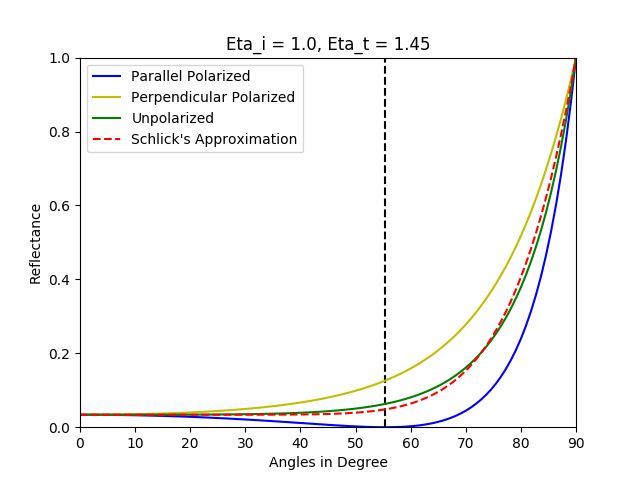
\includegraphics[width = 2.8in]{./CO417_Figure/01.png} 
            \caption{Fresnel and Schlick's Apprx. of $\eta_i$=1.0 and $\eta_t$ = 1.45}
        \end{minipage}
        \begin{minipage}{7cm}
            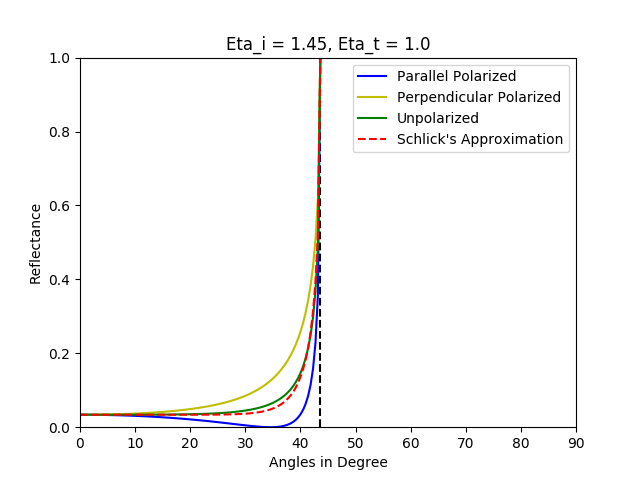
\includegraphics[width = 2.8in]{./CO417_Figure/02.png} 
            \caption{Fresnel and Schlick's Apprx. of $\eta_i$=1.45 and $\eta_t$ = 1.0} 
        \end{minipage}
     
\end{figure}\\
As is shown in Figure 1, the Parallel and Perpendicular Polarized reflectance according to incident angle are plotted as blue and yellow solid curves and the unpolarized reflectance is plotted as green solid curves. For index of refractions in Figure 1, the black dotted line represents Brewster's angle, where $R_{\parallel}=0$, which has a value of $\theta_B = arctan\frac{\eta_t}{\eta_i} = 55.41 (^{\circ})$. For Figure 2, the black dotted line is Critical angle, representing the smallest angle that occurs total internal reflection. The value of Critical andgle in Figure 2 is $\theta_C = arcsin\frac{\eta_t}{\eta_i} = 43.60 (^{\circ})$.\\ 
The Schlick's Approximation is shown in red dotted line and calculated by $F_r(cos\theta)=R_0 + (1-R_0)(1-cos\theta)^5$ with $R_0$ the reflectance at normal incident. According to Figure 1 and 2, it could be concluded that the Schlick's method approximates unpolarized reflectance very well. In addition, the advantage of Schlick's Apprx is to acquire approximated reflactance without estimating index of refractions.

\newpage

\section{Generate MC samples according to an EM}
The second part of the assignment is to generate a number of Monte-Carlo samples from lat-long format environment map Grace Cathedral. The generating method is based on Probability Density Function and Cumulative Density Function. For each pixel in lat-long map, the intensity of the pixel is calculated by $Intensity_{ij} = \frac{R+G+B}{3}$. After that, considering the shape of lat-long format, primitive PDF of each pixel should be scaled by its solid angle $\theta (0-\pi)$: $p(x_{ij}) = Intensity_{ij} * sin\theta$. \\
After the procedure, the 2D PDF of the lat-long EM has been generated. In addition, a 1D PDF that contains sum likelihood of each row is generated for row selection later ($p(r_i) = \sum_1^jp(x_{ij})$). Here, to acquire a proper CDF later, 2D PDF will be normalised as the sum of likelihood of each row equals to 1 ($\sum_1^jp(x_{ij})=1$).The 1D row PDF is normalised as well ($\sum_1^ip(r_{i})=1$).\\
In order to sample from PDF, 1D CDF across rows will be generated next. For each sample, firstly, use uniform random variate $u_i\in [0,1]$ to decide which row to sample. CDF value of row $r_m$ is calculated by $C(r_m) = \sum_1^m p(r_m)$. Apply same operation to rows of 2D PDF to acquire 2D CDF. Given that each likelihood is greater or equal than 0, $C(r_{m+1}) > C(r_{m})$ for each $m$. Therefore, $r_i=C^{-1}(u_i)$ and row number ($i$) of the sample is acquired. Next, generate another uniform random variate $u_j\in [0,1]$ and use the same method to acquire sample column. Extract row $i$ from 2D CDF and $x_{ij} = C^{-1}(u_j)$. For the assignment, 64, 256 and 1024 samples maps are generated corrspondingly.\\
After generation of samples, apply scaling and gamma correction to acquire final output. Here the step=6 and gamma=2.2. For clarity, a 5X5 neighbour window around samples are set to blue alone with samples.\\
For 256 samples, a map only contains sample points and 5X5 windows set to sample RGB values are generated as well.\\


    \begin{figure}[H]
        \centering % this centers the figure
            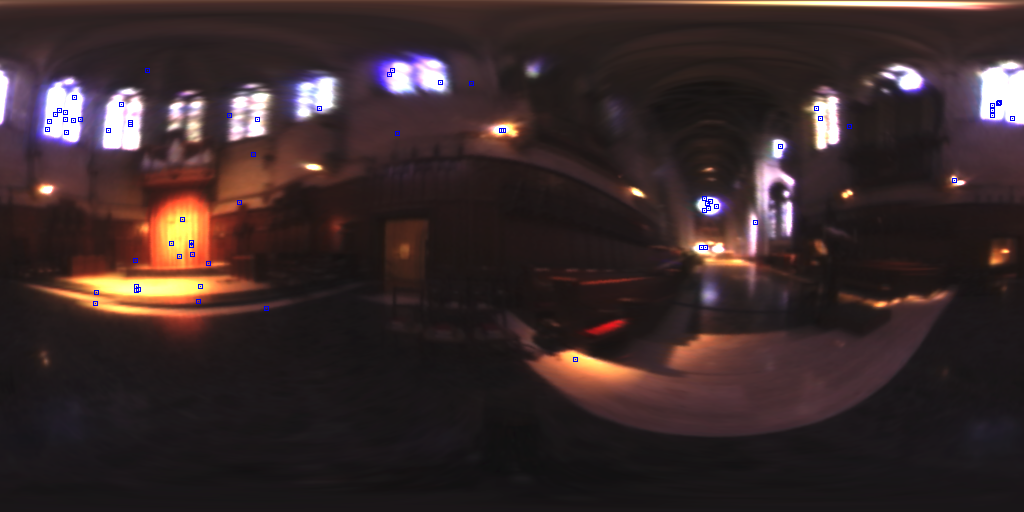
\includegraphics[width = 6in]{./CO417_Figure/MC_64.png} 
            \caption{64 Samples with Grace Cathedral EM} % caption of the figure
            \label{fig:imperial figure} % a label. When we refer to this label from the text, the figure number is included automatically
            
             \end{figure}

            \newpage    
            \begin{figure}[H]
        \centering % this centers the figure
            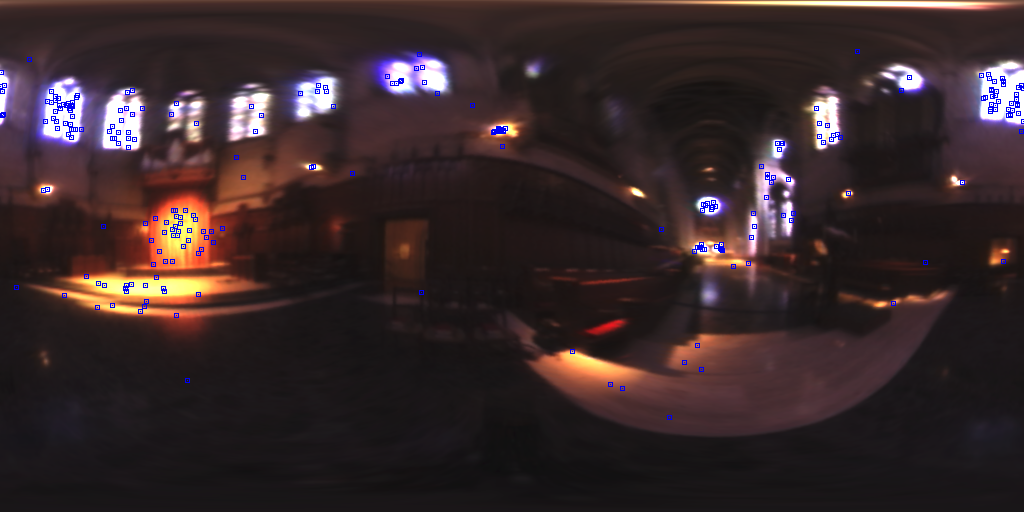
\includegraphics[width = 6in]{./CO417_Figure/MC_256.png} 
            \caption{256 Samples with Grace Cathedral EM} % caption of the figure
            \label{fig:imperial figure} % a label. When we refer to this label from the text, the figure number is included automatically        
 
            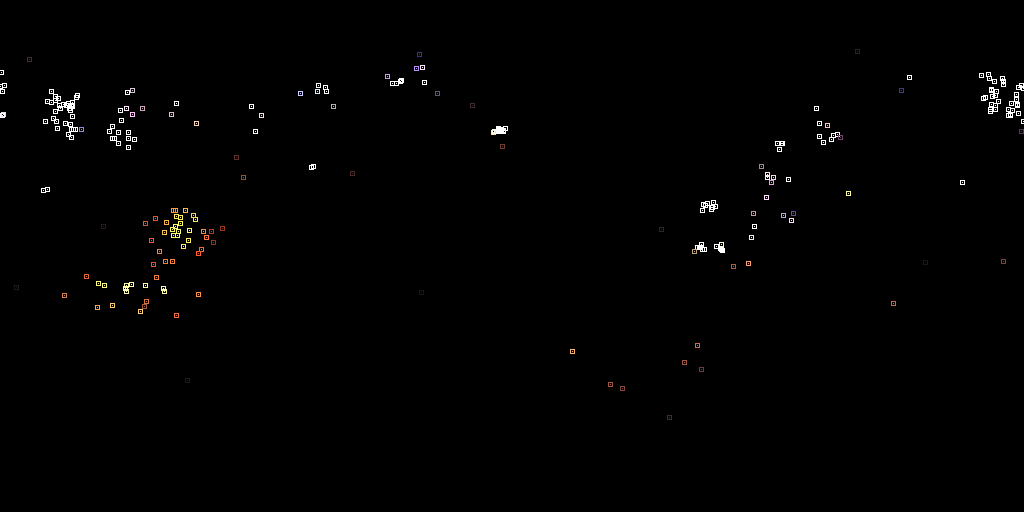
\includegraphics[width = 6in]{././CO417_Figure/SAMPLE_MAP_256.png} 
            \caption{256 Samples extracted from Grace Cathedral EM} % caption of the figure
            \label{fig:imperial figure} % a label. When we refer to this label from the text, the figure number is included automatically

            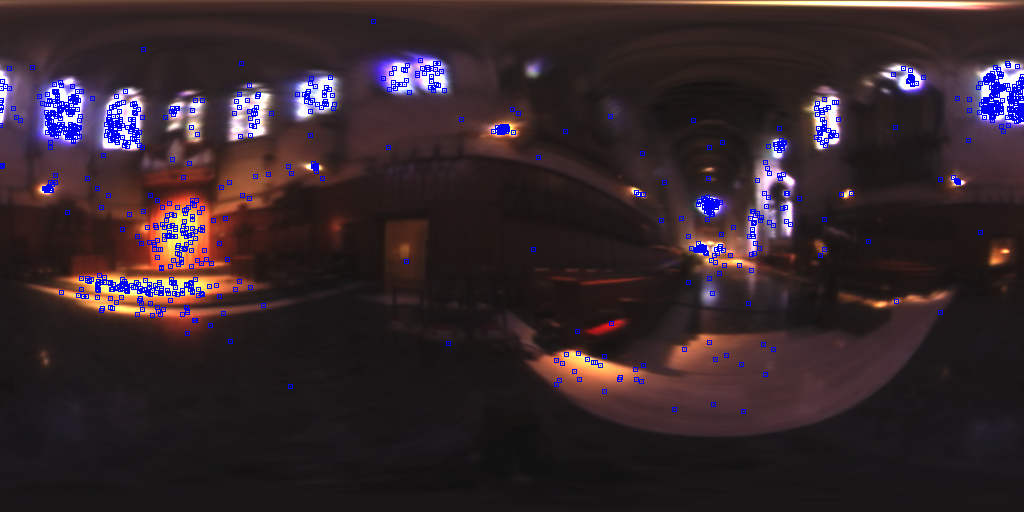
\includegraphics[width = 6in]{././CO417_Figure/MC_1024.png} 
            \caption{1024 Samples with Grace Cathedral EM} % caption of the figure
            \label{fig:imperial figure} % a label. When we refer to this label from the text, the figure number is included automatically
        \end{figure}
        
According to Figure 3 to 6, it can be concluded that comparing to dim pixels, brighter pixels have greater chance to be sampled. Comparing to rows closing to top and ground, rows closing to centre have greater chance to be selected. 
      
\end{document}
%%% Local Variables: 
%%% mode: latex
%%% TeX-master: t
%%% End: 
